\documentclass[11pt,a4paper]{article}
% Preámbulo común de los informes de docs/reports/ (no forma parte de la memoria).
\usepackage[T1]{fontenc}
\usepackage[utf8]{inputenc}
\usepackage[spanish,es-noshorthands,es-tabla]{babel}
\usepackage{lmodern}
\usepackage{microtype}
\usepackage[a4paper,margin=2.3cm]{geometry}
\usepackage{graphicx}
\usepackage{booktabs}
\usepackage{tabularx}
\usepackage{array}
\usepackage{multirow}
\usepackage{amsmath}
\usepackage{enumitem}
\usepackage{float}
\usepackage{adjustbox}
\newcommand{\fittable}[1]{\begin{adjustbox}{max width=\linewidth}\input{#1}\end{adjustbox}}
\usepackage[font=small,labelfont=bf]{caption}
\usepackage[dvipsnames,table]{xcolor}
\usepackage{fancyhdr}
\usepackage[most]{tcolorbox}
\usepackage[hidelinks]{hyperref}

\definecolor{accent}{HTML}{2A78D6}
\definecolor{inkmuted}{HTML}{52514E}
\definecolor{boxbg}{HTML}{F3F6FB}
\definecolor{warnbg}{HTML}{FDF6E7}
\definecolor{warnline}{HTML}{C98500}

\setlist{itemsep=2pt,topsep=4pt}
\setlength{\parindent}{0pt}
\setlength{\parskip}{5pt}
\renewcommand{\arraystretch}{1.12}

\newtcolorbox{keybox}[1][]{colback=boxbg,colframe=accent,boxrule=0.6pt,arc=2pt,
  left=8pt,right=8pt,top=6pt,bottom=6pt,fonttitle=\bfseries,title={#1}}
\newtcolorbox{warnbox}[1][]{colback=warnbg,colframe=warnline,boxrule=0.6pt,arc=2pt,
  left=8pt,right=8pt,top=6pt,bottom=6pt,fonttitle=\bfseries,title={#1}}

\newcommand{\estado}[1]{\textsf{\small\textbf{\color{accent}#1}}}
\newcommand{\ruta}[1]{\texttt{\small #1}}

\pagestyle{fancy}
\fancyhf{}
\renewcommand{\headrulewidth}{0.3pt}
\fancyfoot[C]{\small\color{inkmuted}\thepage}

\fancyhead[L]{\small\color{inkmuted}Resumen para la tutoría}
\fancyhead[R]{\small\color{inkmuted}12 de noviembre de 2026}
\graphicspath{{figures/}}

\title{\textbf{Resumen para la tutoría}\\[2pt]\large Estado del TFG y decisiones pendientes}
\author{TFG «Plataforma para la experimentación con Quantum Machine Learning»}
\date{12 de noviembre de 2026 · commits \texttt{dec0f0b}--\texttt{4424eb7} sobre \texttt{bc877bd}\\
\small Fuente: \ruta{docs/tutor-briefing-2026-11-12.md} y secciones 30--34 de \ruta{docs/TFG-technical-log.md}}

\begin{document}
\maketitle
\thispagestyle{fancy}

Estados usados:
\begin{itemize}
  \item \estado{Propuesto}: solo aparece en un plan.
  \item \estado{Implementado}: el código existe, sin evaluar.
  \item \estado{Validado}: una prueba concreta se ha superado.
  \item \estado{Evaluado}: experimento con resultados persistidos y analizados.
\end{itemize}

\section{Qué se necesita decidir}

\begin{keybox}
\begin{enumerate}[leftmargin=*]
  \item Qué línea de entrenamiento es la \textbf{principal} en la memoria: la variacional (circuito y optimizador
        clásico) o la QGD (actualización de pesos dentro del circuito).
  \item Si se acepta la \textbf{actualización modular} de QGD como sustituta del clipping, y con qué rejilla y qué
        \texttt{b/lr}.
  \item Qué significa «no híbrido» para el TFG: sin PyTorch, sin Adam, o actualización ejecutada como circuito.
  \item Qué resultados serán \textbf{oficiales} en la memoria.
\end{enumerate}
\end{keybox}

\section{Estado en una tabla}

\begin{table}[H]
\centering\small
\begin{tabularx}{\linewidth}{>{\raggedright\arraybackslash}X >{\raggedright\arraybackslash}p{3.2cm} >{\raggedright\arraybackslash}p{4.3cm}}
\toprule
Componente & Estado & Evidencia \\
\midrule
QCNN de 4 qubits (codificación angular y de fase, convolución, pooling lógico) & \estado{Validado} &
  Pruebas unitarias: 124/124 OK el 12-nov (las 3 pruebas nuevas de la fase C pasan por separado) \\
Legado híbrido PyTorch + Adam & \estado{Evaluado} (histórico, $n=3$) & \ruta{results/\allowbreak initial-hybrid-adam/} \\
QGD M1--M5 (actualización modular reversible) & \estado{Validado} unitariamente; \textbf{no evaluado} & Log, secciones 28--30; auditoría \\
Ruido local corregido (matriz de densidad, shots independientes) & \estado{Validado} & Log, sección 30 \\
Línea variacional (GD, Adam, SPSA, secuencial tipo Rotosolve/NFT) & \estado{Evaluado} en simulación & \ruta{results/variational/} (log, secciones 31--34) \\
Ejecución en hardware real (QPU) & \estado{Propuesto} & No hay adaptador, transpilación ni ejecuciones \\
\bottomrule
\end{tabularx}
\end{table}

\section{Problemas encontrados y corregidos (auditoría independiente)}

\begin{itemize}
  \item \textbf{Ninguna ejecución QGD previa movía los pesos.} Con \texttt{b=5} y \texttt{lr=0.1}, el desplazamiento
        entero es 0 para los 32 códigos de gradiente, así que los pesos solo se cuantizan. Por tanto, los perfiles M5 y
        los screens S0/G0/U0 no evalúan QGD como método de entrenamiento. Ahora el código detecta esta situación,
        avisa y la registra en el JSON.
  \item \textbf{Las pruebas de la aritmética QGD eran vacuas}, porque usaban configuraciones con desplazamiento 0. Se
        añadieron pruebas exhaustivas con configuraciones que sí mueven pesos (circuito frente a la referencia
        clásica), y pasan.
  \item \textbf{El ruido estaba mal modelado en Qibo 0.1.11:}
  \begin{itemize}
    \item el canal depolarizante compartía una única trayectoria de ruido entre todos los shots, así que no promediaba realizaciones;
    \item en matriz de densidad, ese mismo canal despolariza todo el registro, no solo el qubit objetivo;
    \item en ejecución repetida, todos los shots reutilizan la muestra del primero.
  \end{itemize}
  Se sustituyó por un canal local exacto. Los JSON antiguos con ruido no son estimaciones promediadas.
  \item \textbf{Las métricas M5 no tenían referencia trivial:} en Iris, la accuracy de test (0,333--0,467) está
        \textbf{por debajo} de la clase mayoritaria (0,533).
\end{itemize}

\section{Resultados de la línea variacional en la partición 42 (\estado{Evaluado} en simulación)}

\textbf{Protocolo:}
\begin{itemize}
  \item Ajuste de hiperparámetros solo con validation (fase A).
  \item Confirmación con 8 semillas de inicialización nuevas y test evaluado una sola vez (fase B), en cuatro
        condiciones: exacta, 1000 shots, 1000 shots con ruido local ($p=0{,}001$) y error de lectura del 2\,\%, y
        presupuesto común de circuitos.
  \item Baselines de clase mayoritaria y regresión logística.
  \item Comparaciones pareadas con IC bootstrap y Wilcoxon.
\end{itemize}

\begin{table}[H]
\centering\small
\begin{tabular}{lccc}
\toprule
Dataset (test) & QCNN, rango de accuracy & Clase mayoritaria & Regresión logística \\
\midrule
Breast Cancer, PCA 4 (86 casos) & 0,846--0,919 & 0,628 & 0,907 \\
Iris setosa/versicolor (15 casos) & 0,858--1,000 & 0,467 & 1,000 \\
\bottomrule
\end{tabular}
\end{table}

La tabla corresponde a la partición 42 (fase B). La fase C (sección~\ref{sec:faseC}), con 10 particiones nuevas, matiza estas lecturas:
\begin{itemize}
  \item La QCNN \textbf{aprende} y supera claramente a la clase mayoritaria. En la partición 42 quedaba a la altura de
        la regresión logística, pero \textbf{con 10 particiones queda por debajo de ella en ambos datasets}.
  \item \textbf{No hay un optimizador consistentemente mejor.} En Breast Cancer, GD, Adam y el secuencial empatan. En
        Iris con codificación angular, GD superó a Adam en la partición 42, pero \textbf{no se replica} con 10 particiones.
  \item \textbf{El optimizador secuencial} (reconstrucción exacta del coste por coordenada) alcanza el mejor checkpoint
        con muchos menos circuitos: entre 3,7 y 23 veces menos que Adam en Breast Cancer y entre 2 y 12 veces menos en
        Iris, sin perder accuracy. Es el único hallazgo que se mantiene en la fase C, y es relevante para el hardware,
        donde el coste se mide en ejecuciones.
  \item \textbf{Los 1000 shots y el ruido de sensibilidad} apenas cambian la accuracy de test (solo se midió en la
        partición 42).
\end{itemize}
\textit{Limitaciones:} simulación en CPU, ruido no calibrado, pocos casos de test en Iris, corrección por
multiplicidad solo en la fase C y sin QPU.

\section{Situación de QGD respecto al objetivo de hardware real}

\textbf{Lo implementado} (\estado{Implementado} y \estado{Validado} unitariamente):
\begin{itemize}
  \item El host calcula el gradiente por parameter-shift a partir de las medidas.
  \item El gradiente se codifica en un registro de $b$ qubits.
  \item Un circuito aritmético reversible suma el desplazamiento al registro del peso (módulo $2^b$).
  \item El resultado se mide y se decodifica.
\end{itemize}

\begin{warnbox}[Limitaciones del diseño, no solo de su evaluación]
\begin{enumerate}[leftmargin=*]
  \item \textbf{La entrada y la salida del circuito de actualización son clásicas.} El gradiente llega ya calculado
        desde el host, y el peso se mide y vuelve al host. El circuito hace una suma modular que el host podría hacer
        directamente: no elimina el bucle ni la actualización clásicos, solo la traslada a un circuito con coste y
        ruido añadidos.
  \item \textbf{Coste en hardware.} Usa puertas multicontroladas de hasta $2b$ qubits
        (\texttt{max\_qubits\_per\_arithmetic\_gate}), que en un dispositivo real habría que descomponer. No hay
        transpilación, routing ni validación de conectividad.
  \item \textbf{Regla de actualización.} La rejilla duplica los extremos $\pm\pi$ y no representa el cero. La regla
        modular no equivale al clipping del plan original, y su aceptación está pendiente.
  \item \textbf{No hay ninguna ejecución QGD con pesos que se muevan}, así que no se puede afirmar nada cuantitativo
        sobre su rendimiento.
\end{enumerate}
\end{warnbox}

Llevar la actualización de pesos al circuito sin ningún paso clásico (por ejemplo, estimando el gradiente de forma
coherente) exigiría algoritmos que en general necesitan hardware tolerante a fallos. Esta afirmación
\textbf{todavía no tiene referencias verificadas} en \ruta{memory/bibliography.bib} y debe tratarse como pendiente de
bibliografía.

\section{Opciones}

\begin{table}[H]
\centering\small
\begin{tabularx}{\linewidth}{>{\raggedright\arraybackslash}p{3.3cm} >{\raggedright\arraybackslash}X >{\raggedright\arraybackslash}p{2.6cm} >{\raggedright\arraybackslash}p{3.3cm}}
\toprule
Opción & Qué implica & Coste & Riesgo \\
\midrule
\textbf{A.} Variacional como línea principal; QGD como prototipo documentado &
  Memoria con resultados evaluados (fases B y C). QGD se presenta como exploración de la actualización en circuito,
  con sus límites y sin cifras de rendimiento. &
  Bajo: los experimentos ya están hechos & Se aparta de la intención inicial de «actualización en circuito» \\
\addlinespace
\textbf{B.} QGD como línea principal &
  Fijar un \texttt{b/lr} que mueva pesos, corregir la rejilla, decidir la política de decodificación y evaluar QGD
  con el mismo protocolo (pareado frente a la variacional). &
  Medio-alto: implementación y experimentos & Es probable que no supere a la variacional; la limitación 1 persiste \\
\addlinespace
\textbf{C.} Ambas, con comparación controlada &
  A, más una evaluación de QGD con una configuración que mueva pesos y el mismo protocolo. &
  Medio & Alcance mayor; requiere decidir antes la regla QGD \\
\bottomrule
\end{tabularx}
\end{table}

\begin{keybox}[Recomendación técnica]
Opción \textbf{A}, o \textbf{C} si el tutor considera imprescindible una cifra de QGD. En ambos casos, el paso de
mayor valor hacia el «hardware real» sería una ejecución pequeña de la línea variacional en un proveedor de QPU (por
ejemplo, la inferencia de un checkpoint entrenado).
\end{keybox}

\section{Fase C: robustez frente a la partición}\label{sec:faseC}

\estado{Evaluado} en simulación exacta.

\textbf{Diseño}, pre-registrado antes de ejecutar:
\begin{itemize}
  \item 10 particiones nuevas por dataset (semillas 1--10) $\times$ 4 optimizadores $\times$ 2 codificaciones
        $\times$ 8 semillas de inicialización: 1280 entrenamientos.
  \item Hiperparámetros de la fase A, sin reajuste.
  \item Unidad de análisis: la partición, con corrección de Holm.
  \item Fuente: \ruta{results/variational/C-partitions/README.md} y \ruta{analysis.md}.
\end{itemize}

\begin{table}[H]
\centering\small
\begin{adjustbox}{max width=\linewidth}
\begin{tabular}{lcccc}
\toprule
Accuracy de test (media $\pm$ sd) & Mejor QCNN & Peor QCNN & Logística & Mayoritaria \\
\midrule
Breast Cancer & 0,911 $\pm$ 0,022 (Adam, angular) & 0,853 $\pm$ 0,034 (SPSA, fase) & 0,937 $\pm$ 0,018 & 0,628 \\
Iris & 0,928 $\pm$ 0,060 (secuencial, angular) & 0,817 $\pm$ 0,145 (GD, fase) & 1,000 $\pm$ 0,000 & 0,500 \\
\bottomrule
\end{tabular}
\end{adjustbox}
\end{table}

\begin{figure}[H]
\centering
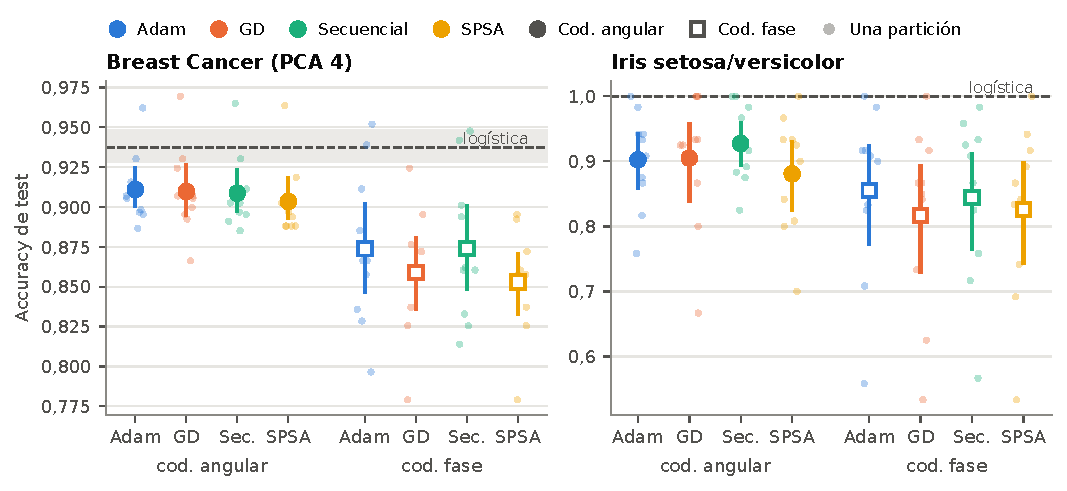
\includegraphics[width=\linewidth]{fig04_phaseC_accuracy.pdf}
\caption{Accuracy de test en 10 particiones por dataset. Los puntos pequeños son la media de cada partición; el
marcador grande, la media con su IC95\,\%. La línea discontinua es la regresión logística.}
\end{figure}

\textbf{Qué se mantiene y qué no:}
\begin{enumerate}
  \item \textbf{Optimizadores:} ninguna diferencia de accuracy frente a Adam es significativa tras Holm. En Iris, la
        variación entre particiones (sd 0,06--0,14) supera cualquier diferencia entre optimizadores.
  \item \textbf{GD mejor que Adam en Iris: no se replica} ($+0{,}003$, IC $[-0{,}038,\ 0{,}040]$). Era propio de la partición 42.
  \item \textbf{SPSA peor que Adam y angular mejor que fase en Breast Cancer:} misma dirección que en la fase B, pero
        sin significación tras Holm ($p=0{,}059$ y $0{,}074$).
  \item \textbf{El secuencial es más barato en circuitos en las 40 combinaciones} de partición, dataset y
        codificación (Holm $p=0{,}014$): necesita entre 3,2 y 9,4 veces menos circuitos hasta el checkpoint.
  \item \textbf{QCNN frente a regresión logística:} queda por debajo en casi todas las particiones, de $-0{,}026$ a
        $-0{,}084$ en Breast Cancer y de $-0{,}07$ a $-0{,}18$ en Iris. La partición 42 era favorable a la QCNN.
  \item \textbf{Parada temprana (patience)}, reconstruida del historial:
  \begin{itemize}
    \item Con $P=10$ para todos, el secuencial para con el 14--19\,\% de los circuitos de 100 pasos y no pierde accuracy.
    \item Adam con $P=10$ pierde hasta 0,032 en Iris.
    \item Con esa regla, el secuencial consume entre 1,2 y 2,2 veces menos circuitos que Adam hasta parar.
  \end{itemize}
\end{enumerate}

\begin{keybox}[Lectura para la decisión de la sección 1]
La línea variacional está evaluada de forma reproducible. Lo que se puede defender no es que la QCNN supere al
clasificador clásico, sino que:
\begin{enumerate}[leftmargin=*]
  \item aprende, por encima de la clase mayoritaria;
  \item queda por debajo de una regresión logística con las mismas 4 características;
  \item el optimizador secuencial reduce el número de ejecuciones del circuito sin perder accuracy, lo que importa en hardware.
\end{enumerate}
Esto refuerza la opción A. Para la memoria convendría tomar como oficiales los resultados de la fase C (varias
particiones) y presentar los de la fase B como un caso concreto. El informe
\ruta{docs/reports/variational-results.pdf} recoge todas las gráficas y tablas.
\end{keybox}

\section{Fuentes en el repositorio}

\begin{itemize}
  \item \ruta{docs/TFG-technical-log.md}: secciones 28--34.
  \item \ruta{docs/experimental-protocol.md}: protocolo variacional.
  \item README de cada fase, en \ruta{results/variational/}:
  \begin{itemize}
    \item \ruta{A-tuning-bc-exact/} y \ruta{B-confirm-bc/};
    \item \ruta{B-confirm-iris/} y \ruta{C-partitions/}.
  \end{itemize}
  \item \ruta{results/quantum-training/}: perfiles M5, con pesos que no se mueven.
  \item Auditoría independiente: \ruta{AUDIT.md}, en el paquete de traspaso, fuera del repositorio.
\end{itemize}

\end{document}
